\subsection{History}


One of the main features of \alida is the capability of automatically documenting data processing
pipelines. 
The operator concept allows for automatically logging all data manipulations,
which can subsequently be used to convert the
processing history into a directed graph data structure, denoted {\em processing
graph} in the following.
 
The \alida\ operator concept defines operators as the only places where data are processed and manipulated. 
Each invocation of an operator is associated with a certain configuration of the operator, defined by the values of its \icode{IN} and \icode{INOUT} parameters.
A data analysis pipeline usually consists of a set of different operators that are applied to incoming data and
produce result data. The order in which the operators work on the data depends on the specific pipeline as well as on the input data. The invocation of
operators can be of pure sequential nature or subsume parallel processing steps. In addition, a nested application
of operators is possible. Given these principles, each analysis pipeline and its
data flow may be interpreted
and visualized as a directed acyclic graph (cf.~Fig.~\ref{fig:DAG2} for an
example).

\begin{figure}[t]
\begin{center}
\centerline{{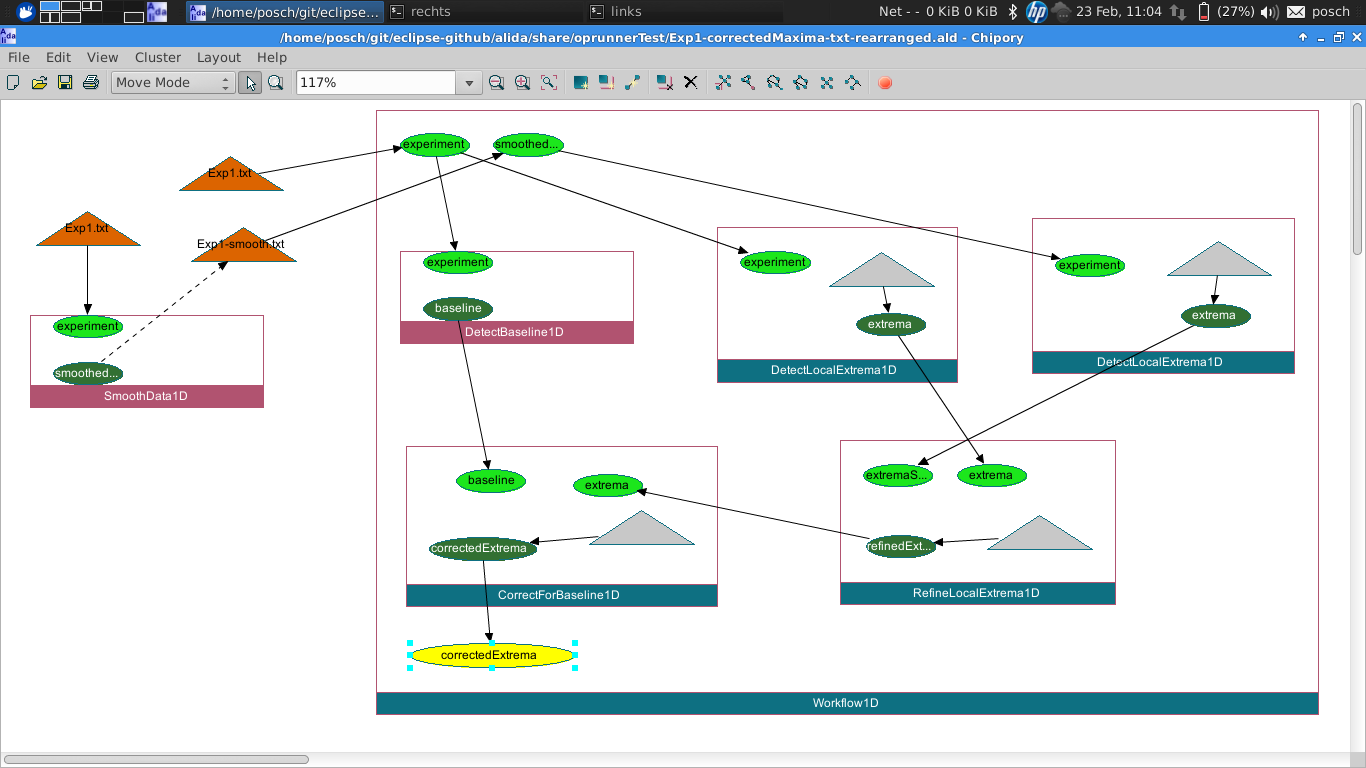
\includegraphics[clip, trim= 10 40 30 90, width=\textwidth]{Exp1-correctedMaxima-txt-rearranged.png}}}
\end{center}
\vspace*{-0.75cm}
\caption[Example of a processing graph.]{\label{fig:DAG2}
A processing graph: the directed acyclic graph represents the application of nested operators. 
Calls to operators are depicted as rectangles, input and output ports as ellipses filled in light or dark green,
respectively. 
The yellow ellipse indicates the result data object
to which this processing graph is linked to.
The triangles relate to newly generated data objects which are colored in grey
unless the data object was read from file.
In this case the triangle is colored orange.}
\end{figure}

The processing graph is stored in XML format in a file accompanying the actual data object file. 
The format basically relies on {\em GraphML}\footnote{GraphML website, 
\href{http://graphml.graphdrawing.org/}{http://graphml.graphdrawing.org/}} with some \alida 
specific extensions. 
If the history is stored externally when a data object is written to disk
depends in general on the data type.
However, when invoking operators from the command line user interface,
most \alida data types will write a history if output of a parameter is
redirected to a file.
\alida uses the
extension \icode{'.ald'} for an {\em \alida\ processing graph} file.
The same is true when reading data.
I.e., in general it depends on the data type if a history is read from file, if
existing. The command line user interface will do this in most cases.

Note, the identity of data is {\em not} preserved in the processing history
across file boundaries. If two (or more) input data for the current top
level operator are loaded
from the same file, both will nevertheless be displayed as different data
nodes in the history. The reason is that object identity is not -- and maybe even cannot -- be checked from the
processing history of former operations.

A processing graph basically consists of operator and data nodes which are connected by edges 
indicating the flow of data, as can be seen from Fig.~\ref{fig:DAG2}. 
The figure shows a screenshot of \mtbc which is a graph visualization tool derived from {\em Chisio}
(see Appendix~\ref{app:chipory} for details).
Within the processing graph each operator node, which is linked to the {\em invocation} of a specific operator,
is depicted as a rectangle with the operator's 
classname in the bottom line.
For each input and output parameter object the operator node features input and output ports which may be conceived as the entry or exit points of data into and out of the operator. These ports are depicted as filled ellipses in light green (input ports) and dark green (output ports),
respectively. Each input port has exactly one incoming edge, while an output
port may be connected to multiple target ports,
depending on where the data is passed to. 
Each port of an operator has an individual name indicating the input or output object associated
with the port. 

In addition to operator nodes and their ports there are also data nodes in the
graph, corresponding to the creation of new data objects, e.g., when data is read from
file, cloned or generated from scratch. These are depicted as triangles filled
in light grey in most cases.
If data is read from file, the triangle is tagged by a string
and colored orange.
%%If the
%%data object extends the class \icode{ALDData} this string gives the name of the file
%%the data was read from. 
If in addition
a processing graph of a
former analysis procedure was read, this history is also included into the
processing graph
and connected by a dashed edge (see top left part of Fig.~\ref{fig:DAG2}).


